% --------------------------------------------------------------------------------

\begin{exercise}

Formulieren und beweisen Sie das Lemma $3.8$ explizit für den Fall $m=2$.

\end{exercise}

% --------------------------------------------------------------------------------

\begin{solution}

\begin{figure}[h!]
  \centering
  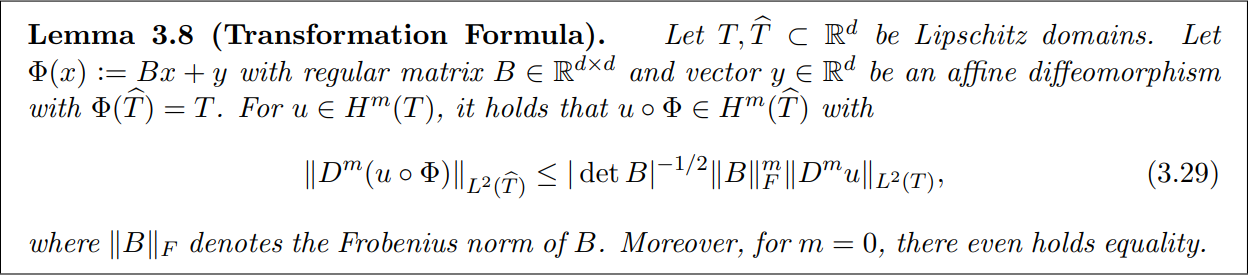
\includegraphics
  [width = 0.75 \textwidth]
  {NumPDEs/NumPDEs - Lemma 3.8 (Transformation Formula).png}
\end{figure}

\begin{align*}
  \Psi:
  C^\infty(\overline T) \to H^2(\hat T):
  u \mapsto u \circ \Phi
\end{align*}

Wir zeigen zuerst die Wohldefiniertheit von $\Psi$ als linearer und
beschränkter Operator, d.h. $\Exists C > 0:$

\begin{align*}
  \norm[H^2(\hat T)]{\Psi u}
  \leq
  C \norm[H^2(T)]{u}.
\end{align*}

Dazu zeigen wir zunächst die Transformationsfomel für $u \in C^{\infty}(\overline{T})$ und $m = 0,1,2$.

\begin{enumerate}[label = \arabic*.]

  \item Abschätzung ($m = 0$):
  Die steht sogar explizit im Skript.

  \begin{align*}
    \implies
    \norm[L^2(T)]{u}^2
    =
    \Int[T]{u^2}{y}
    =
    \Int[\hat T]{(u \circ \Phi)^2 |\det D \Phi|}{x}
    =
    |\det B| \norm[L^2(\hat T)]{u \circ \Phi}^2
  \end{align*}

  \item Abschätzung ($m = 1$):

  \begin{align*}
    \implies
    \partial_j (u \circ \Phi)(x)
    =
    \sum_{n=1}^d
    \partial_n u(\Phi(x)) B_{nj}
  \end{align*}

  Jetzt verwenden wir die Cauchy-Schwarz-Bunjakovski Ungleichung.

  \begin{align*}
    \implies
    |\partial_j (u \circ \Phi)(x)|^2
    & \stackrel
    {
      \mathrm{CSB}
    }
    {\leq}
    \pbraces
    {
      \sum_{n=1}^d
      \partial_n u(\Phi(x))|^2
    }
    \pbraces
    {
      \sum_{n=1}^d
      B_{nj}^2
    }
    =
    |Du(\Phi(x))|^2
    \pbraces
    {
      \sum_{n=1}^d
      B_{nj}^2
    }
    \end{align*}

  Jetzt verwenden wir die Transformationsfomel.

  \begin{align*}
    \implies
    |\det B| \norm[L^2(\hat T)]{D(u \circ \Phi)}^2
    & =
    \Int[\hat T]
    {
      \sum_{j=1}^d
      |\partial_j (u \circ \Phi)(x)|^2
      |\det D \Phi(x)|
    }{x} \\
    & \leq
    \Int[\hat T]
    {
      \sum_{j=1}^d
      |Du(\Phi(x))|^2
      \pbraces
      {
        \sum_{n=1}^d
        B_{nj}^2
      }
      |\det D \Phi(x)|
    }{x} \\
    & =
    \sum_{j=1}^d
    \pbraces
    {
      \sum_{n=1}^d
      B_{nj}^2
    }
    \Int[\hat T]
    {
      |Du(\Phi(x))|^2
      |\det D \Phi(x)|
      }{x} \\
    & \stackrel
    {
      \mathrm{TRAFO}
    }{=}
    \sum_{j=1}^d
    \pbraces
    {
      \sum_{n=1}^d
      B_{nj}^2
    }
    \Int[T]
    {
      |Du(x)|^2
    }{x} \\
    & =
    \norm[F]{B}^2 \norm[L^2(T)]{Du}^2
  \end{align*}

  \item Abschätzung ($m = 2$):

  \begin{align*}
    \implies
    D(u \circ \Phi) = Du(\Phi(x))D\Phi(x) = Du(\Phi(x))B
  \end{align*}

  \begin{align*}
    \implies
    \partial_k \partial_j (u \circ \Phi)(x)
    &=
    \partial_k \pbraces
    {
      \sum_{n=1}^d
      \partial_n u(\Phi(x)) B_{nj}
    } \\
    &=
    \sum_{n=1}^d
    B_{nj} \partial_k (\partial_n u(\Phi(x)))
    =
    \sum_{n=1}^d
    \sum_{m=1}^d
    \partial_m \partial_n u(\Phi(x)) B_{nj} B_{mk}
  \end{align*}

  Jetzt verwenden wir Cauchy-Schwarz-Bunjakovski.

  \begin{align*}
    \implies
    |\partial_k \partial_j (u \circ \Phi)(x)|^2
    &\stackrel
    {
      \mathrm{CSB}
    }
    {\leq}
    \pbraces
    {
      \sum_{n,m=1}^d
      |\partial_m \partial_n u(\Phi(x))|^2
    }
    \pbraces
    {
      \sum_{n,m=1}^d |B_{nj} B_{mk}|^2
    } \\
    &=
    |D^2 u(\Phi(x))|^2
    \pbraces
    {
      \sum_{n=1}^d
      B_{nj}^2
    }
    \pbraces
    {
      \sum_{m=1}^d
      B_{mk}^2
    }
  \end{align*}

  Jetzt verwenden wir die Transformationsfomel.

  \begin{align*}
    \implies
    |\det B| \norm[L^2(\hat T)]{D^2(u\circ\Phi)}^2
    & =
    \Int[\hat T]
    {
      \sum_{j=1}^d
      \sum_{k=1}^d
      |\partial_k \partial_j (u \circ \Phi)(x)|^2
      |\det D\Phi(x)|
    }{x} \\
    & \leq
    \Int[\hat T]
    {
      \sum_{j=1}^d
      \sum_{k=1}^d
      |D^2 u (\Phi(x))|^2
      \pbraces
      {
        \sum_{n=1}^d
        B_{nj}^2
      }
      \pbraces
      {
        \sum_{m=1}^d
        B_{mk}^2
      }
      |\det D \Phi(x)|
    }{x} \\
    & =
    \sum_{j=1}^d
    \sum_{k=1}^d
    \pbraces
    {
      \sum_{n=1}^d
      B_{nj}^2
    }
    \pbraces
    {
      \sum_{m=1}^d
      B_{mk}^2
    }
    \Int[\hat T]
    {
      |D^2 u (\Phi(x))|^2
      |\det D \Phi(x)|
    }{x} \\
    & \stackrel
    {
      \mathrm{TRAFO}
    }{=}
    \sum_{j=1}^d
    \sum_{k=1}^d
    \pbraces
    {
      \sum_{n=1}^d
      B_{nj}^2
    }
    \pbraces
    {
      \sum_{m=1}^d
      B_{mk}^2
    }
    \Int[T]{|D^2 u(x)|^2}{x} \\
    & =
    \pbraces
    {
      \sum_{j=1}^d
      \sum_{n=1}^d
      B_{nj}^2
    }
    \pbraces
    {
      \sum_{k=1}^d
      \sum_{m=1}^d
      B_{mk}^2
    }
    \norm[L^2(T)]{D^2 u}^2 \\
    & =
    \norm[F]{B}^4 \norm[L^2(T)]{D^2 u}^2.
  \end{align*}

\end{enumerate}

Mit diesen Abschätzungen bekommen wir die Stetigkeit von $\Psi$, d.h. $\Exists C > 0:$

\begin{multline*}
  \norm[H^2(\hat T)]{\Psi u}
  =
  \norm[H^2(\hat T)]{u \circ \Phi}
  =
  \norm[L^2(\hat T)]{u \circ \Phi}^2
  +
  \norm[L^2(\hat T)]{D (u \circ \Phi)}^2
  +
  \norm[L^2(\hat T)]{D^2 (u \circ \Phi)}^2 \\
  \leq
  |\det B|^{-1/2}
  \pbraces
  {
    \norm[L^2(T)]{u}^2
    +
    \norm[F]{B}^2
    \norm[L^2(T)]{Du}^2
    +
    \norm[F]{B}^4
    \norm[L^2(T)]{D^2 u}^2
  }
  \leq
  C^2 \norm[H^2(T)]{u}^2.
\end{multline*}

Als nächstes erweitern wir das Resultat mit Dichtheitsargumenten auf den ganzen $H^2(T)$.

$C^{\infty}(\overline{T})$ liegt ja dicht in $H^2(T)$.
$\Phi$ kann somit (eindeutig) stetig auf dem ganzen Raum $H^2(T)$ fortgesetzt werden
(sogar normerhaltend).

Wir wollen nun zeigen, dass für $\Forall u \in H^2(T):$

\begin{align*}
  \Psi u = u \circ \Phi.
\end{align*}

Sei dazu $u \in H^2(T)$ und $(u_n)_{n \in \N} \subset C^{\infty}(\overline{T})$ mit

\begin{align*}
  u_n \xrightarrow[n \to \infty]{H^2(T)} u.
\end{align*}

Aufgrund der $\norm[H^2]{\cdot}$-Stetigkeit von $\Psi$, erhalten wir damit auch

\begin{align*}
  \implies
  u_n \circ \Phi = \Psi(u_n) \xrightarrow[n \to \infty]{H^2(T)} \Psi u.
\end{align*}

Weil $\norm[L^2]{\cdot} \leq \norm[H^2]{\cdot}$, erhalten wir für $(u_n)_{n \in \N}$ auch $L^2(T)$-Konvergenz.

\begin{align*}
  \implies
  u_n \xrightarrow[n \to \infty]{L^2(T)} u
\end{align*}

Weil $u$ messbar ist, können wir die Transformationsformel darauf anwenden.
Die 1. Abschätzung ($m = 0$) liefert uns also

\begin{align*}
  u_n \circ \Phi \xrightarrow[n \to \infty]{L^2(\hat T)} u \circ \Phi.
\end{align*}

Weil Grenzwerte eindeutig sind, folgt unsere Behauptung.

\begin{align*}
  \implies
  u \circ \Phi = \Psi u
\end{align*}

Nun ist jede Norm $\norm{\cdot}$ in sich selbst stetig ($\norm{\cdot}$-stetig), und

\begin{align*}
  u_n \xrightarrow[n \to \infty]{H^2(T)} u,
  \quad
  u_n \circ \Phi \xrightarrow[n \to \infty]{H^2(\hat T)} u \circ \Phi.
\end{align*}

Ähnlich wie vorher gilt $\norm[L^2]{D^2 (\cdot)} \leq \norm[H^2]{\cdot}$.

\begin{align*}
  \implies
  D^2 u_n \xrightarrow[n \to \infty]{L^2(T)} D^2 u,
  \quad
  D^2 (u_n \circ \Phi) \xrightarrow[n \to \infty]{L^2(\hat T)} D^2 (u \circ \Phi)
\end{align*}


\begin{align*}
  \implies
  \norm[L^2(\hat T)]{D^2(u\circ\Phi)}
  &=
  \lim_{n \to \infty}
  \norm[L^2(\hat T)]{D^2(u_n\circ\Phi)} \\
  &\leq
  \lim_{n \to \infty}
  |\det B|^{-1/2}
  \norm[F]{B}^2
  \norm[L^2(T)]{D^2 u_n}
  =
  |\det B|^{-1/2}
  \norm[F]{B}^2
  \norm[L^2(T)]{D^2 u}
\end{align*}

\end{solution}

% --------------------------------------------------------------------------------
